\lstset{language=bash}
\newpage
\chapter{Design} % (30-40 pages)
% 
% TODO: Reconsider the formatting of this introduction
In this chapter, we examine various data structures and algorithms with key aspects that may make them suitable for incorporation into a \lstinline{Version Control System}.\\
% TODO: Decide whether to include this paragraph or not due to the top paragraph of the "Data Structures" section (see below)
% \\This examination evaluates several alternative data structures, including \lstinline{Linked Lists}, \lstinline{Binary Trees}, \lstinline{Hash Tables}, and \lstinline{Directed Acyclic Graphs (DAGs)}, focusing on their operational efficiency, structural properties, and implementation considerations.
% Furthermore, algorithms for functionality such as \lstinline{Traversal} and \lstinline{Difference (Diffing)} are analyzed in terms of their computational complexity, conceptual simplicity, and implementation considerations.\\\\
% Finally, the chapter also assesses what metrics are relevant to facilitate the comparison of these data structures and algorithms.
We also assess what metrics are relevant to facilitate the comparison of these data structures and algorithms.
% 
% ------------------------------------------------------------------------------
% 
% TODO: Change title
\section{Data Structures}
% Data Structures
% ---------------
% TODO: Add references
Data structures are objects that can be used to store, organize, and manipulate large amounts of data. They play a crucial role in computer science and are fundamental building blocks of many software systems, including \lstinline{Version Control Systems}. The choice of data structure is critical to the overall performance and scalability of a \lstinline{Version Control System}.

In order to evaluate the suitability of a data structure for implementation in a \lstinline{Version Control System}, it is necessary to consider several core aspects. Firstly, \lstinline{operational efficiency}, which refers to the time and space complexity of the basic operations performed by the data structure, is a crucial consideration. The efficiency of these operations can have a significant impact on the overall performance of the \lstinline{Version Control System}.

Another important aspect is the data structure's \lstinline{structural specificity}, which encompasses how data is stored and organized within the structure. This is critical because the structural specifics can affect the ease of implementation and the ability to efficiently perform operations such as \lstinline{insertions}, \lstinline{deletions}, and \lstinline{updates}.

Lastly, the \lstinline{implementation details} must be considered, including the ease of implementation and compatibility with the programming language. A data structure that is straightforward to implement and easy to maintain/iterate upon will result in a more streamlined and efficient \lstinline{Version Control System}.
% 
% What are the potential data structures that could be used?
%  - Explain the data structures in detail - (4 x 2 page)
%  - Explain the pros and cons of each data structure - (4 x 0.5 page)
%  - Explain how each data structure will be implemented - (4 x 1 page)
% 
% TODO: Add references
\subsection{Linked List}
% ------------------------------------------------------------------------------
% TODO: Add explanation of why a linked list is suitable for a Version Control System
% ------------------------------------------------------------------------------
A \lstinline{Linked List} is a linear collection of data elements, called nodes, each pointing to the next node by means of a pointer. The \lstinline{Linked List} is the most sought-after data structure when it comes to handling dynamic data elements \cite{ravikiran_2022}.

There are two main types of \lstinline{Linked Lists}: \lstinline{Singly-Linked Lists (SLL)} and \lstinline{Doubly-Linked Lists (DLL)}, but we will only be considering the \lstinline{Doubly-Linked List (DLL)} when we reach the \lstinline{Implementation} chapter.
% TODO: Fix spacing between these two paragraphs
% There are two types of \lstinline{Linked Lists}:
\paragraph{Singly-linked lists (SLL)}
% Singly-Linked List Definition
\begin{itemize}
    \item \lstinline{SLL} nodes contain two fields: \lstinline{data} field and \lstinline{next} pointer field.
    \item Traversal of a \lstinline{SLL} can be done using the \lstinline{next} pointer field only. Meaning, the \lstinline{SLL} can be traversed in only one direction, from the first node to the last node.
    \item The \lstinline{SLL} occupies less memory than a \lstinline{DLL} because it does not contain a \lstinline{prev} pointer field.
    \item \lstinline{SLL} is preferred over \lstinline{DLL} when it comes to the execution of stack and queue operations.
    \item \lstinline{SLL} is also preferred over \lstinline{DLL} to save memory when a searching operation is not required.
\end{itemize}
% Singly-Linked List Efficiency Analysis
\begin{table}[h]
    \centering
    \caption{Efficiency Analysis of Singly-Linked List Operations}
    \label{tab:singly-linked-list-efficiency-analysis}
    \begin{tabular}{|c|c|c|}
        \hline
        Operation           & Worst Case & Average Case \\ \hline
        Access              & $O(n)$     & $O(n)$       \\ \hline
        Search              & $O(n)$     & $O(n)$       \\ \hline
        Insert              & $O(n)$     & $O(n)$       \\ \hline
        Insert (at Head)    & $O(1)$     & $O(1)$       \\ \hline
        Insert (at Current) & $O(1)$     & $O(1)$       \\ \hline
        Insert (at Tail)    & $O(1)$     & $O(1)$       \\ \hline
        Delete              & $O(n)$     & $O(n)$       \\ \hline
        Delete (at Head)    & $O(1)$     & $O(1)$       \\ \hline
        Delete (at Current) & $O(n)$     & $O(n)$       \\ \hline
        Delete (at Tail)    & $O(n)$     & $O(n)$       \\ \hline
    \end{tabular}
\end{table}
% Singly-Linked List Diagram
\begin{figure}[!htbp]
    \centering
    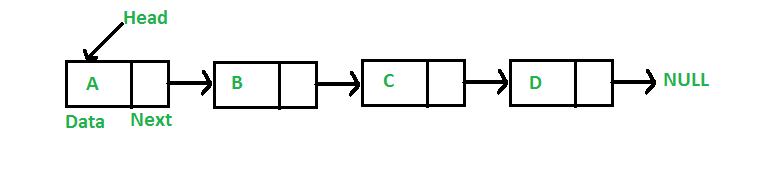
\includegraphics[width=0.9\textwidth]{singly-linked-list.png}
    \caption{Singly Linked List (SLL) \cite{vaghani_2023}}
    \label{fig:singly-linked-list}
\end{figure}

\paragraph{Doubly-linked lists (DLL)}
% Doubly-Linked List Definition
\begin{itemize}
    \item \lstinline{DLL} nodes contain three fields: \lstinline{data} field, \lstinline{prev} pointer field and \lstinline{next} pointer field.
    \item Traversal of a \lstinline{DLL} can be done using the \lstinline{next} pointer field or the \lstinline{prev} pointer field. Meaning, the \lstinline{DLL} can be traversed in both directions, from the first node to the last node and vice versa.
    \item The \lstinline{DLL} occupies more memory than a \lstinline{SLL} because it contains a \lstinline{prev} pointer field.
\end{itemize}
% Doubly-Linked List Efficiency Analysis
\begin{table}[h]
    \centering
    \caption{Efficiency Analysis of Doubly-Linked List Operations}
    \label{tab:doubly-linked-list-efficiency-analysis}
    \begin{tabular}{|c|c|c|}
        \hline
        Operation           & Worst Case & Average Case \\ \hline
        Access              & $O(n)$     & $O(n)$       \\ \hline
        Search              & $O(n)$     & $O(n)$       \\ \hline
        Insert              & $O(n)$     & $O(n)$       \\ \hline
        Insert (at Head)    & $O(1)$     & $O(1)$       \\ \hline
        Insert (at Current) & $O(1)$     & $O(1)$       \\ \hline
        Insert (at Tail)    & $O(1)$     & $O(1)$       \\ \hline
        Delete              & $O(n)$     & $O(n)$       \\ \hline
        Delete (at Head)    & $O(1)$     & $O(1)$       \\ \hline
        Delete (at Current) & $O(1)$     & $O(1)$       \\ \hline
        Delete (at Tail)    & $O(1)$     & $O(1)$       \\ \hline
    \end{tabular}
\end{table}
% Doubly-Linked List Diagram
\begin{figure}[!htbp]
    \centering
    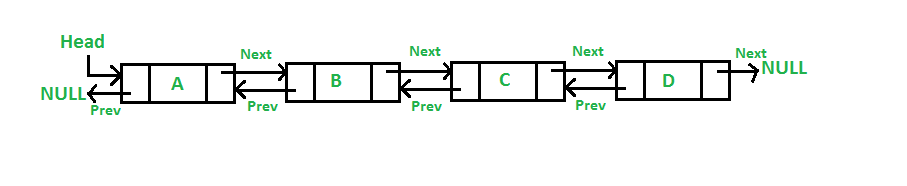
\includegraphics[width=1.1\textwidth]{doubly-linked-list.png}
    \caption{Doubly Linked List (DLL) \cite{vaghani_2023}}
    \label{fig:doubly-linked-list}
\end{figure}
% TODO: Check positioning of the figure
\newpage
% 
% TODO: Add references
% Advantages and Disadvantages in the context of a Version Control System
\paragraph{Advantages}
\begin{itemize}
    \item Dynamic size: As new versions of a file are created, the \lstinline{Linked List} can grow in size to accommodate the new data, without the need to pre-allocate memory.
    \item Efficient storage of file changes: Each node in the \lstinline{Linked List} can store the entire contents of a file version, along with metadata such as the date and time the change was made. This allows for efficient storage of file changes over time.
    \item Easy traversal of file history: The \lstinline{Linked List} structure allows for easy traversal of the file history, as each node contains a reference to the previous version of the file. This makes it easy to track changes and revert to previous versions of a file.
    \item Memory efficient: The \lstinline{Linked List} structure is memory efficient, as each node only contains the current version of the file and changes made to it, along with simple references to the next and previous nodes in the list. This means that the \lstinline{Linked List} structure does not need to store the entire file history in memory, which can be a significant amount of data.
\end{itemize}
\paragraph{Disadvantages}
\begin{itemize}
    \item Inefficient retrieval of specific file versions: Retrieving a specific version of a file can be slow, as the \lstinline{Linked List} structure does not allow for random access to the file history. This means that the entire file history must be traversed from the most recent version of the file to the desired version.
    \item Limited scalability: For large file histories, the \lstinline{Linked List} structure can be less efficient and will not scale as well as other data structures.
    \item Extra memory overhead: Each node in the \lstinline{Linked List} structure contains a reference to the next and previous nodes in the list, which can add up when dealing with large file histories.
    \item Not suitable for concurrent access: The \lstinline{Linked List} structure is not suitable for concurrent access, as it is not thread-safe and can lead to data corruption and race conditions.
\end{itemize}

% TODO: Add implementation details
\paragraph{Implementation Details}
Exercitation ullamco culpa velit excepteur aute esse amet. Quis adipisicing consequat quis sunt elit cupidatat sunt ipsum nostrud laborum aliqua veniam veniam commodo. Minim ullamco aute aliquip eiusmod officia cillum fugiat magna consectetur aute sunt aliqua labore. Reprehenderit dolore commodo deserunt laborum culpa laborum elit. Labore Lorem quis culpa amet adipisicing pariatur consequat eu proident in officia aute voluptate. Excepteur irure deserunt et ullamco deserunt labore anim dolor amet est est culpa. Magna eiusmod nulla ipsum esse anim nostrud mollit fugiat proident magna laboris.

Ut non aliquip aliquip Lorem reprehenderit nisi qui aliqua cupidatat enim adipisicing deserunt. Eiusmod est dolore ut ipsum Lorem et sunt est minim in Lorem. Reprehenderit ea proident officia anim dolore incididunt sunt labore sunt. Ea sunt incididunt anim tempor. Esse amet ut magna id irure ex.

Id do cillum ad ad officia dolor sunt deserunt amet ex. Pariatur aute sint anim aute id irure reprehenderit laboris non tempor id. Labore in ad sunt nulla dolore velit ut aliquip amet dolore quis voluptate nisi. Magna non magna nulla officia magna voluptate officia dolore Lorem ea sunt duis. Non dolore proident voluptate consequat consequat laborum aliqua veniam et occaecat amet ea dolore.

% TODO: Add references
\paragraph{Summary}
A \lstinline{Doubly-Linked List} is a data structure that consists of a sequence of nodes, each node having a data field and two pointers, one pointing to the next node in the list and the other pointing to the previous node.

One of the main advantages of using a \lstinline{Doubly-Linked List} is that it allows for easy insertion and deletion of nodes, making it possible to add new file versions or remove outdated ones easily.

However, Concurrent access to a \lstinline{Doubly-Linked List} can lead to data inconsistencies and race conditions, and proper synchronization must be implemented to prevent these issues.

\subsection{Binary Tree}
% ------------------------------------------------------------------------------
% TODO: Add explanation of why a binary tree is suitable for a Version Control System
% ------------------------------------------------------------------------------
A \lstinline{Binary Tree} is a hierarchical data structure that consists of a set of nodes, where each node can have at most two children. The topmost node in the tree is called the root node, and the nodes that do not have any children are called leaf nodes. The nodes that have children are called internal nodes. The \lstinline{Binary Tree} structure is a special case of the \lstinline{Tree} data structure, where each node can have at most two children.

Each node in a \lstinline{Binary Tree} contains the following elements:
\begin{enumerate}
    \item Data: The data stored in the node.
    \item Left child: A pointer to the left child node.
    \item Right child: A pointer to the right child node.
\end{enumerate}

% TODO: Add references/Confirm this is correct
There are several different types of \lstinline{Binary Tree} structures, including:
\begin{enumerate}
    \item Full Binary Tree: A \lstinline{Binary Tree} where each node has either zero or two children.
    \item Complete Binary Tree: A \lstinline{Binary Tree} where all levels of the tree are completely filled, except for the last level. The last level of the tree is filled from left to right.
    \item Balanced Binary Tree: A \lstinline{Binary Tree} where the difference between the height of the left and right subtrees of any node is not greater than one.
    \item Degenerate (or Pathological) Binary Tree: A \lstinline{Binary Tree} that is not balanced, where the height of the tree is equal to the number of nodes in the tree.
\end{enumerate}

% Binary Tree Efficiency Analysis
\begin{table}[h]
    \centering
    \caption{Efficiency Analysis of Binary Tree Operations}
    \label{tab:binary-tree-efficiency-analysis}
    \begin{tabular}{|c|c|c|}
        \hline
        Operation & Worst Case & Average Case \\ \hline
        Search    & $O(n)$     & $O(\log n)$  \\ \hline
        Insert    & $O(n)$     & $O(\log n)$  \\ \hline
        Delete    & $O(n)$     & $O(\log n)$  \\ \hline
    \end{tabular}
\end{table}
% TODO: Add image of binary tree data structure
\begin{figure}[!htbp]
    \centering
    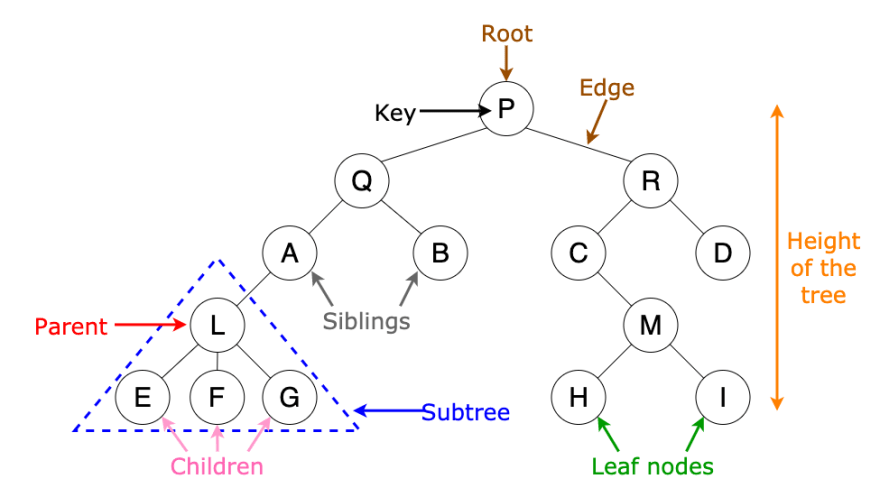
\includegraphics[width=0.8\textwidth]{binary-tree.png}
    \caption{Binary Tree \cite{mcmahon_2020}}
    \label{fig:binary-tree}
\end{figure}
\newpage
% TODO: Add binary tree detailed efficiency analysis of each operation

% TODO: Add references
% Advantages and Disadvantages in the context of a Version Control System
\paragraph{Advantages}
\begin{itemize}
    \item Efficient storage of file changes: Each node in the \lstinline{Binary Tree} structure can store the entire contents of a file version, along with metadata such as the date and time the version was created. This allows for efficient storage of file changes, as the entire file history can be stored in a single \lstinline{Binary Tree} structure.
    \item Easy traversal of file history: The \lstinline{Binary Tree} structure allows for easy traversal of the file history, with the root node representing the most recent version of the file and the leaf nodes representing the oldest versions of the file. This makes it easy to track changes and revert to previous versions of the file.
    \item Flexibility: \lstinline{Binary Tree} structures can be used to implement a variety of other data structures, such as \lstinline{Binary Search Trees}, \lstinline{AVL Trees}, \lstinline{Heaps}, and others, which can be useful for other operations in a \lstinline{Version Control System}.
\end{itemize}
% TODO: Confirm this is correct
\paragraph{Disadvantages}
\begin{itemize}
    \item Inefficient retrieval of specific file versions: The \lstinline{Binary Tree} structure can be slow when retrieving specific file versions, as it requires traversing the \lstinline{Binary Tree} to find the desired node. This can be inefficient when dealing with large file histories.
    \item Limited scalability: For large file histories, the \lstinline{Binary Tree} structure can be less efficient and may not scale as well as other data structures.
    \item Extra memory overhead: Each node in the \lstinline{Binary Tree} structure requires extra memory to store the pointers to the left and right child nodes. This can become significant when dealing with large file histories.
    \item Unbalanced trees can lead to poor performance: If the \lstinline{Binary Tree} structure becomes skewed, the time complexity of searching, insertion, and deletion operations can become \lstinline{O(n)}, where \lstinline{n} is the number of nodes in the tree.
    \item Not suitable for concurrent access: The \lstinline{Binary Tree} structure is not suitable for concurrent access, as it is not thread-safe. This can lead to data corruption and race conditions.
\end{itemize}

% TODO: Add implementation details
\paragraph{Implementation Details}
Nulla cillum laborum quis et cillum eu. Id exercitation ad aliquip ipsum elit excepteur tempor occaecat enim excepteur culpa aliqua ullamco pariatur. Et do elit nisi duis et aliquip consequat dolor labore.

Laborum consequat elit fugiat excepteur esse exercitation anim anim est eiusmod aliquip ad. Labore veniam cillum officia aute elit minim minim in laboris. Incididunt velit amet consequat officia nulla exercitation ex voluptate in duis ullamco Lorem.

Nostrud officia consectetur proident aliquip elit commodo do pariatur eu aliqua. Commodo irure deserunt tempor nisi cillum elit nulla dolore amet pariatur aliquip irure reprehenderit aute. Cillum minim cillum irure commodo cillum eu consequat et dolore sint sunt aliquip fugiat consequat. In laboris exercitation fugiat aute laboris mollit cupidatat laboris nostrud ut. Non enim aliquip anim ullamco non incididunt proident eu. Et officia tempor exercitation magna incididunt incididunt veniam reprehenderit.

% TODO: Summary of the suitability of the data structure in the context of a Version Control System
\paragraph{Summary}
Magna fugiat consectetur magna adipisicing minim id elit Lorem culpa. Ut cillum adipisicing fugiat pariatur consectetur irure. Sit voluptate mollit nulla culpa incididunt minim velit non ex nostrud ad. Amet eiusmod magna voluptate nulla exercitation sit id. Nostrud in do id exercitation excepteur minim reprehenderit anim excepteur veniam eiusmod duis proident. Eiusmod aliquip laborum deserunt officia cillum Lorem excepteur Lorem ad.

\subsection{Hash Table}
% ------------------------------------------------------------------------------
% TODO: Add explanation of why a hash table is suitable for a Version Control System
% ------------------------------------------------------------------------------
A \lstinline{Hash Table} is a data structure that uses a hash function to map keys to their corresponding values. It is an efficient way to implement an associative array, where keys are used to look up values.

The basic idea behind a \lstinline{Hash Table} is to use a hash function to map a key to an index in an array, called a bucket, where the corresponding value can be found or stored. The process of mapping a key to an index is called \lstinline{hashing}.

Each element in a \lstinline{Hash Table} consists of:
\begin{enumerate}
    \item Key: This is the value used to look up a corresponding element in the \lstinline{Hash Table}.
    \item Value: This is the value associated with the key that is stored in the \lstinline{Hash Table}.
\end{enumerate}

% TODO: Add references
When a new element is added to a \lstinline{Hash Table}, the key is passed through a \lstinline{hash} function which produces an \lstinline{index} (also called a hash value or bucket) where the element is stored.
When a value is to be retrieved, the key is passed through the same hash function, and the resulting \lstinline{index} is used to look up the corresponding value in the \lstinline{Hash Table}.

% Hash Table Efficiency Analysis
\begin{table}[h]
    \centering
    \caption{Efficiency Analysis of Hash Table Operations}
    \label{tab:hash-table-efficiency-analysis}
    \begin{tabular}{|c|c|c|}
        \hline
        Operation & Worst Case & Average Case \\ \hline
        Search    & $O(n)$     & $\Theta(1)$  \\ \hline
        Insert    & $O(n)$     & $\Theta(1)$  \\ \hline
        Delete    & $O(n)$     & $\Theta(1)$  \\ \hline
    \end{tabular}
\end{table}
% Image of hash table data structure
\begin{figure}[!htbp]
    \centering
    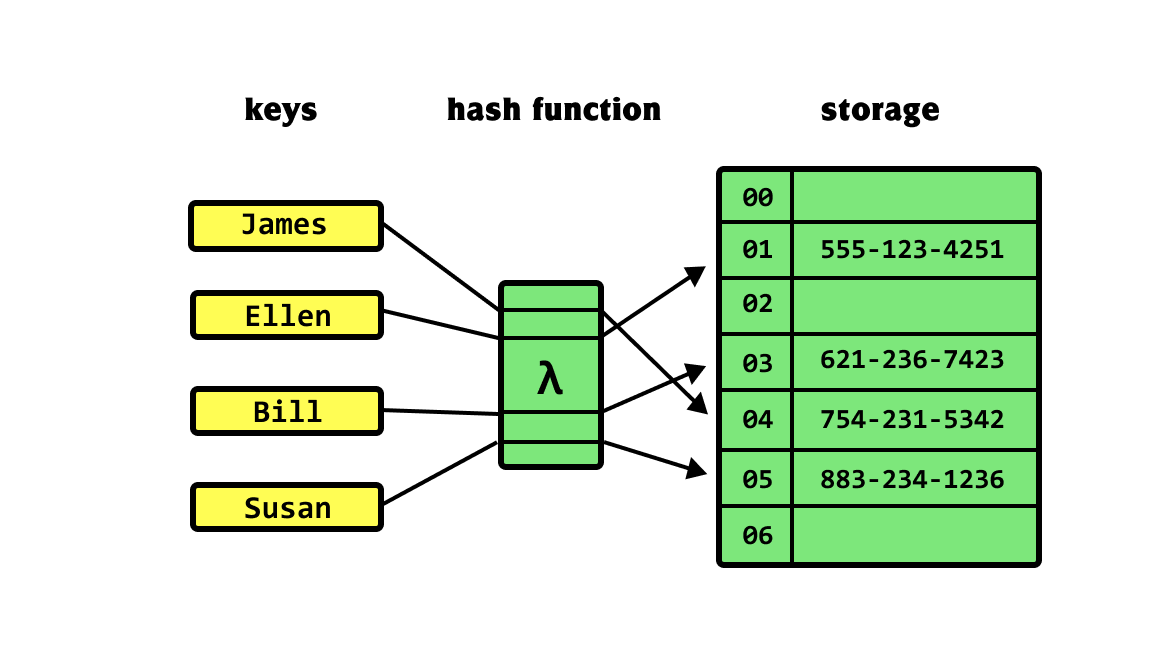
\includegraphics[width=0.8\textwidth]{hash-table.png}
    \caption{Hash Table \cite{stemmler_2022}}
    \label{fig:hash-table}
\end{figure}
\newpage
% TODO: Add hash table detailed efficiency analysis of each operation

% TODO: Add references
% Advantages and Disadvantages in the context of a Version Control System
\paragraph{Advantages}
\begin{itemize}
    \item Efficient searching, insertion, and deletion: A well-implemented \lstinline{Hash Table} allows for these operations to be performed in \lstinline{O(1)} time, which is useful for a Version Control System as it needs to be able to quickly retrieve, insert, and delete file versions.
    \item Dynamic resizing: \lstinline{Hash Tables} can grow or shrink in size as needed, which is useful for a Version Control System as the number of file versions can vary greatly.
          % TODO: Confirm that this is true
    \item Low overhead: A \lstinline{Hash Table} only requires a small amount of overhead for pointers and the hash function, and thus uses less memory than an array or a \lstinline{Linked List} with the same number of elements.
\end{itemize}
\paragraph{Disadvantages}
\begin{itemize}
    \item{Hash collisions: \lstinline{Hash} functions can produce collisions, where two different keys produce the same \lstinline{index}, leading to the same location in the \lstinline{Hash Table}.}
    \begin{itemize}
        \item{\lstinline{Collision resolution techniques}, such as \lstinline{open addressing} and \lstinline{separate chaining}, can be used to handle collisions but it still increases the time complexity of the \lstinline{Hash Table} operations.}
    \end{itemize}
    \item Clustering: When all the elements in a \lstinline{Hash Table} are stored in the same bucket, it is called \lstinline{clustering}. This can lead to a performance degradation leading the \lstinline{Hash Table} operations to have the worst-case time complexity of \lstinline{O(n)} for insertion, deletion, and retrieval.
\end{itemize}

% TODO: Add implementation details
\paragraph{Implementation Details}
Non veniam nostrud occaecat magna minim officia fugiat ad tempor nulla sunt laboris deserunt minim. Officia commodo ut anim culpa dolore eiusmod ex do tempor tempor Lorem dolore aute culpa. Fugiat aliqua tempor minim esse consequat cupidatat sint dolor mollit irure consectetur fugiat. Ipsum excepteur eu cillum ea sit cillum sunt excepteur exercitation fugiat Lorem ut fugiat ut. Nulla aliquip cillum pariatur dolore aute pariatur do. Excepteur labore veniam eiusmod dolore dolor mollit eu.

Ea aliqua incididunt consectetur id officia. Dolor enim commodo pariatur enim veniam anim. Culpa laboris eu aute anim aliquip. Voluptate laboris et minim labore exercitation aliqua.

Quis voluptate duis dolore ea proident duis et ad. Proident sunt irure sint minim veniam ut laboris culpa laboris eiusmod id. Duis proident id nulla dolor est dolore. Mollit exercitation ad eiusmod ad eiusmod duis occaecat fugiat elit occaecat eu. Incididunt nisi velit quis mollit dolore cupidatat qui fugiat labore in. Est do qui enim in adipisicing eiusmod pariatur enim sit exercitation dolore officia.

% TODO: Summary of the suitability of the data structure in the context of a Version Control System
\paragraph{Summary}
Minim non consequat culpa eu officia aliquip officia officia veniam in. Velit ut Lorem ea do adipisicing velit aliquip laborum. Proident dolore pariatur aliquip excepteur consectetur culpa adipisicing enim irure tempor eiusmod. Deserunt minim aliquip occaecat cillum mollit. In nulla fugiat consectetur nisi aliquip incididunt proident excepteur ex excepteur voluptate laboris. Reprehenderit amet anim incididunt aliqua est minim labore ipsum duis consectetur amet. Do mollit quis eiusmod ad consectetur ea nulla dolore voluptate nisi ea laborum est.

\subsection{Directed Acyclic Graph (DAG)}
% ------------------------------------------------------------------------------
% TODO: Add explanation of why a DAG is suitable for a Version Control System
% ------------------------------------------------------------------------------
A \lstinline{Directed Acyclic Graph (DAG)} is a type of graph that consists of a set of nodes and directed edges between pairs of nodes. The edges have direction and they connect one node to another.
Unlike in a \lstinline{Tree} structure, in a \lstinline{DAG}, a node can have multiple parents and multiple children, but there cannot be any cycles in the graph.

A node in a \lstinline{DAG} can represent any type of data, and the edges can represent any type of relationship between the nodes. Each node in a \lstinline{DAG} contains the following elements:
\begin{enumerate}
    \item Data: The data that the node represents.
    \item Adjacency list: A list of the nodes that are connected to the current node by an edge.
\end{enumerate}

% Directed Acyclic Graph (DAG) Efficiency Analysis
\begin{table}[h]
    \centering
    \caption{Efficiency Analysis of Directed Acyclic Graph (DAG) Operations}
    % TODO: Create a table of the efficiency analysis of the DAG operations !IMPORTANT!
    \label{tab:dag-efficiency-analysis}
    \begin{tabular}{|c|c|c|}
        \hline
        Operation & Worst Case & Average Case \\ \hline
        % Search    & $O(n)$     & $\Theta(1)$  \\ \hline
        % Insert    & $O(n)$     & $\Theta(1)$  \\ \hline
        % Delete    & $O(n)$     & $\Theta(1)$  \\ \hline
    \end{tabular}
\end{table}
% Image of DAG data structure
\begin{figure}[!htbp]
    \centering
    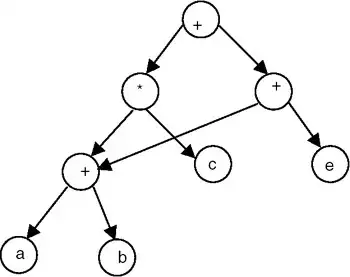
\includegraphics[width=0.8\textwidth]{dag.png}
    \caption{Hash Table \cite{stemmler_2022}}
    \caption{Directed Acyclic Graph (DAG) \cite{surti_2016}}
    \label{fig:dag}
\end{figure}
\newpage
% TODO: Add DAG detailed efficiency analysis of each operation

% TODO: Add references
% Advantages and Disadvantages in the context of a Version Control System
\paragraph{Advantages}
\begin{itemize}
    \item Representing complex relationships: \lstinline{DAGs} can be useful for representing complex relationships between different versions of a file, such as \lstinline{branching} and \lstinline{merging} of changes.
          % TODO: Reconsider this point
    \item Representing multiple paths: \lstinline{DAGs} can be used to represent multiple paths or multiple possibilities of how a file can change over time.
          % TODO: Reconsider this point
    \item Flexibility: \lstinline{DAGs} are very flexible and can be used to represent any type of data and any type of relationship between the data.
\end{itemize}
\paragraph{Disadvantages}
\begin{itemize}
    \item Complex traversal: Traversing a \lstinline{DAG} can be more complex than traversing a \lstinline{Tree} because there can be multiple paths to traverse, which makes it more difficult to retrieve specific versions of a file.
    \item Limited scalability: \lstinline{DAGs} may not scale well for large file histories and a large number of versions because they can become very complex and difficult to traverse.
    \item Not good for searching, insertion, and deletion: \lstinline{DAGs} are not good for searching, insertion, and deletion because they are not ordered and they do not have a root node. This means that the time complexity of these operations is \lstinline{O(n)} due to the need to traverse the entire graph.
\end{itemize}

% TODO: Add implementation details
\paragraph{Implementation Details}
Qui ea velit dolor cupidatat esse anim est labore. Reprehenderit veniam quis magna Lorem ad id exercitation mollit pariatur culpa officia. Dolor commodo aute eu quis Lorem ea nulla eu reprehenderit elit proident. Aliquip nostrud consequat laboris velit anim id dolor fugiat. Aute ea cupidatat velit sunt mollit id proident nostrud incididunt dolore incididunt aliquip adipisicing. Cillum et labore anim est incididunt laborum dolore commodo ullamco mollit ut ut ullamco.

Est veniam aliquip non mollit. Duis aliqua pariatur in officia cillum labore excepteur aliqua nisi. Tempor adipisicing commodo consequat occaecat ad mollit ad fugiat aliquip consectetur aliquip fugiat et. Sunt voluptate exercitation sunt esse.

Ex pariatur labore mollit labore amet. Occaecat culpa commodo ad cillum occaecat voluptate Lorem officia. Deserunt ea velit consequat sunt ex velit cillum do. Dolor nostrud in veniam laboris pariatur fugiat Lorem. Est quis sint anim deserunt elit fugiat culpa occaecat est in anim sunt ipsum.

% TODO: Summary of the suitability of the data structure in the context of a Version Control System
\paragraph{Summary}
Minim ullamco duis officia fugiat anim ad in ipsum adipisicing nostrud mollit exercitation duis cupidatat. Esse occaecat enim anim aliqua qui fugiat mollit deserunt. Lorem culpa laborum ut veniam culpa in nulla et irure. Tempor nostrud magna qui sunt magna aliquip nisi qui. Magna excepteur pariatur mollit sint. Minim non officia aliquip qui laboris sunt. Exercitation aute adipisicing occaecat duis laboris.

% ------------------------------------------------------------------------------

% Algorithms
% ---------------
% What is the essential core functionality of the VCS? (Traversal/Searching, Hashing, Diffing, etc.) - (0.5 page)
% For each functionality, what are the different algorithms that could be used?
% - Explain the algorithms in detail - ((3 x 2) x 1.5 = 9 page)
% - Explain the pros and cons of each algorithm - ((3 x 2) x 0.5 = 3 page)
% - Explain how each algorithm will be implemented - ((3 x 2) x 1 = 6 page)

% What data structures pair well with each algorithm? - (2 page)

% What metrics are important regarding each data structure and algorithm?

% ------------------------------------------------------------------------------

\section{Algorithms}

% TODO: Add intro paragraph



% TODO: Explain the core functionality of the VCS that require algorithms (Traversal/Searching, Hashing, Diffing, etc.)

% ------------------------------------------------------------------------------

\subsection{Traversal}

% TODO: Explain what traversal is and why it is important in a VCS

% TODO: Fill in !important
\subsubsection{Algorithm 1}

% TODO: Fill in !important
\subsubsection{Algorithm 2}

% ------------------------------------------------------------------------------

\subsection{Hashing}

% TODO: Explain what hashing is and why it is important in a VCS

% TODO: Fill in !important
\subsubsection{Algorithm 1}

% TODO: Fill in !important
\subsubsection{Algorithm 2}

% ------------------------------------------------------------------------------

\subsection{Diffing}

% TODO: Explain what diffing is and why it is important in a VCS

% TODO: Fill in !important
\subsubsection{Algorithm 1}

% TODO: Fill in !important
\subsubsection{Algorithm 2}